\section{Experimentos e resultados}

\subsection{Considerações generais}
	\subsubsection{Formulas}
		Para cada uma das redes se calculou todas suas probabilidades usando a propriedade seguinte:
			\[ P( X_i , \ldots , X_n ) = \prod_{i=1}^{n} P( X_i \mid {Pa}( X_i ) ) \]
		Onde ${Pa}( X_i )$ são todas características que são pais de $X_i$ na rede bayesiana. Além disso, a probabilidade condicional pode ser calculada da seguinte forma:
			\[ P( A \mid B ) = \frac{ P( A \cap B ) }{ P( B ) }\]
		Mas para calcular todas as probabilidades, se tem que evaluar cada variável $X_i$ com os valores que aparecem os dados de entrada sendo a fórmula da seguinte forma:
			\[ P( A = a \mid B = b ) = \frac{ N( A = a \cap B = b ) + \alpha_{ab} }{N( B = b ) + \alpha_b } \]
		Para este trabalho os valores de $\alpha$ foram uma estimação com base nos dados calculada com a formula:
			\[ \alpha_{a} = \frac{ 1 }{ |\Omega_a|} \]
		Na formula anterior, se $a$ fosse um conjunto de variáveis, o fator debaixo da fração muda para uma produtora de $\Omega_i$.
	
	\subsubsection{Algoritmo}
		A seguinte lista mostra os parâmetros usados para a busca da melhor rede bayesiana e os valores que foram considerados para todos os experimentos:
		\begin{itemize}
			\item Número de ordens topológicas geradas: 100
			\item Número máximo de pais: O número que tem a rede feita manualmente e 3 para a busca com os dados reais
			\item Número de re-starts: 10
		\end{itemize}
		Então para construir uma rede foram geradas ordens topológicas e para cada característica se fiz uma busca dos melhores pais que pode ter dada essa ordem topológica (os possíveis pais só foram as características anteriores a ela). O número de vezes que foi feito a busca dos melhores pais é igual ao número de re-starts.

\subsection{Experimento 1: Corretude do algoritmo}
\label{subsec:exp1}
	Para poder testar que o algoritmo faz o que diz foi testado com os modelos feitos manualmente e especificados na seção~\ref{sec:construcao}. O objetivo do experimento foi usar o algoritmo para fazer uma busca de redes bayesianas e que a rede usada para gerar os dados seja encontrada entre as melhores. Caso contrario, o algoritmo não está correto.
	\\
	Usando as probabilidades calculadas para cada rede feita manualmente foram gerados dados de treinamento e de teste com a mesma proporção especificada em~\ref{subsec:dadosprop} tendo em total 30 mil dados para cada uma.
	\\
	Na tabela~\ref{tab:loglike} mostra o parâmetro Data Log-Likelihood com os dados de teste gerados para cada uma e também o valor do parâmetro usando os dados reais.
	\begin{table}[ h ]
		\centering
		\begin{tabular}{ | c | c | c | }
			\hline
			Rede & Real Data & Synthetic Data \\ \hline
			1 & -163794.41 & -123773.44 \\ \hline
			2 & -178879.85 & -116475.45 \\ \hline
			3 & -180462.16 & -132307.87 \\ \hline
		\end{tabular}
		\caption{Data Log-Likelihood para cada rede}
		\label{tab:loglike}
	\end{table}
	Os valores são diferentes entre os dois conjuntos de dados porque a quantidade de dados é diferente, mas a proporção entre os valores é similar. A figura~\ref{fig:corretude} mostra as mudanças do valor do parâmetro BIC Score em cada iteração do algoritmo.
	\begin{figure}[H]
		\centering
		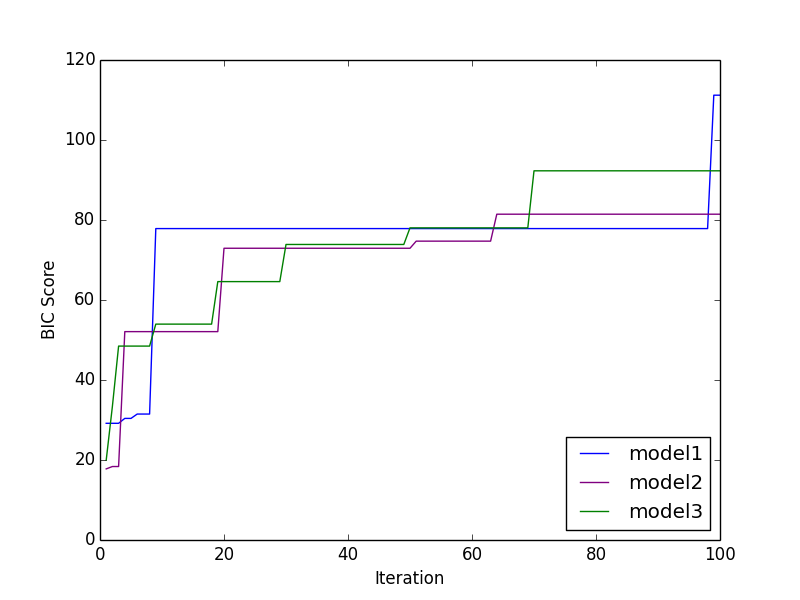
\includegraphics[height=8cm]{images/synt_data}
		\caption{BIC Score (em milhares) para cada rede}
		\label{fig:corretude}
	\end{figure}
	Por último, o algoritmo encontrou a rede bayesiana usada para gerar os dados em todos os casos, mas nenhuma foi a melhor encontrada, mas sem muito cercana. As figuras~\ref{fig:rede1algo},~\ref{fig:rede2algo} e~\ref{fig:rede3algo} mostram as redes que o algoritmo encontrou para cada conjunto de dados.
	\begin{figure}[H]
		\centering
		\begin{tikzpicture}
	\tikzset{ vertex/.style = { shape = circle , draw , minimum size = 2.5em } }
	\tikzset{ edge/.style = { ->,> = latex' } }
	
	% vertices
	\node[ vertex ] (M) at ( 3 , 0 ) { ${M}$ } ;
	\node[ vertex ] (W) at ( 6 , 0 ) { ${W}$ } ;
	
	\node[ vertex ] (ED) at ( 0 , -4 ) { ${ED}$ } ;
	\node[ vertex ] (N) at  ( 1.5 , -4 ) { ${N}$ } ;
	\node[ vertex ] (H) at ( 3 , -4 ) { ${H}$ } ;
	\node[ vertex ] (CG) at ( 4.5 , -4 ) { ${CG}$ } ;
	\node[ vertex ] (CL) at ( 6 , -4 ) { ${CL}$ } ;
	\node[ vertex ] (EN) at  ( 7.5 , -4 ) { ${EN}$ } ;
	\node[ vertex ] (RE) at ( 9 , -4 ) { ${RE}$ } ;

	\node[ vertex ] (AG) at  ( 0 , -8 ) { ${AG}$ } ;
	\node[ vertex ] (AI) at ( 2.25 , -8 ) { ${AI}$ } ;	
	\node[ vertex ] (O) at ( 4.5 , -8 ) { ${O}$ } ;
	\node[ vertex ] (RA) at ( 6.75 , -8 ) { ${RA}$ } ;
	\node[ vertex ] (S) at  ( 9 , -8 ) { ${S}$ } ;
	
	%edges
	%age:annual-income
	\draw[ edge ] (AG) to (AI) ;
	%education-num:
	%sex:
	%native-country:education, age, annual-income
	\draw[ edge ] (N) to (ED) ;
	\draw[ edge ] (N) to (AG) ;
	\draw[ edge ] (N) to (AI) ;
	%education:age, annual-income, occupation, sex, race, relationship
	\draw[ edge ] (ED) to (AI) ;
	\draw[ edge ] (ED) to (O) ;
	\draw[ edge ] (ED) to (S) ;
	\draw[ edge ] (ED) to (RA) ;
	\draw[ edge ] (ED) to[in=135,out=45] (RE) ;
	%relationship:
	%marital-status:workclass, capital-gain, hours-per-week, capital-loss, native-country, education, age, occupation, education-num, race
	\draw[ edge ] (M) to (W) ;
	\draw[ edge ] (M) to (CG) ;
	\draw[ edge ] (M) to (H) ;
	\draw[ edge ] (M) to (CL) ;
	\draw[ edge ] (M) to (N) ;
	%race:
	%workclass:capital-gain, hours-per-week, capital-loss, native-country, education, education-num, relationship
	\draw[ edge ] (W) to (CG) ;
	\draw[ edge ] (W) to (H) ;
	\draw[ edge ] (W) to (CL) ;
	\draw[ edge ] (W) to (N) ;
	\draw[ edge ] (W) to (ED) ;
	\draw[ edge ] (W) to (EN) ;
	\draw[ edge ] (W) to (RE) ;
	%hours-per-week:native-country, occupation, race
	\draw[ edge ] (H) to (N) ;
	\draw[ edge ] (H) to (O) ;
	\draw[ edge ] (H) to (RA) ;
	%occupation:sex
	\draw[ edge ] (O) to[in=-135,out=-45] (S) ;
	%capital-gain:hours-per-week, capital-loss, relationship
	\draw[ edge ] (CG) to (H) ;
	\draw[ edge ] (CG) to (CL) ;
	\draw[ edge ] (CG) to[in=-135,out=-45] (RE) ;
	%capital-loss:education-num
	\draw[ edge ] (CL) to (EN) ;
	%annual-income:sex
	\draw[ edge ] (AI) to[in=-135,out=-45] (S) ;
\end{tikzpicture}
		\caption{Melhor rede para o modelo 1}
		\label{fig:rede1algo}
	\end{figure}
	\begin{figure}[H]
		\centering
		\begin{tikzpicture}
	\tikzset{ vertex/.style = { shape = circle , draw , minimum size = 2.5em } }
	\tikzset{ edge/.style = { ->,> = latex' } }
	% vertices
	\node[ vertex ] (S) at  ( 0 , 0 ) { ${S}$ } ;
	\node[ vertex ] (AG) at  ( 3 , 0 ) { ${AG}$ } ;
	\node[ vertex ] (N) at  ( 6 , 0 ) { ${N}$ } ;
	\node[ vertex ] (EN) at  ( 9 , 0 ) { ${EN}$ } ;
	
	\node[ vertex ] (RE) at ( 0 , -2 ) { ${RE}$ } ;
	\node[ vertex ] (M) at ( 3 , -2 ) { ${M}$ } ;
	\node[ vertex ] (RA) at ( 6 , -2 ) { ${RA}$ } ;
	\node[ vertex ] (ED) at ( 9 , -2 ) { ${ED}$ } ;
	
	\node[ vertex ] (H) at ( 1.5 , -4 ) { ${H}$ } ;
	\node[ vertex ] (W) at ( 4.5 , -4 ) { ${W}$ } ;
	\node[ vertex ] (O) at ( 7.5 , -4 ) { ${O}$ } ;
	
	\node[ vertex ] (CG) at ( 3 , -6 ) { ${CG}$ } ;
	\node[ vertex ] (CL) at ( 6 , -6 ) { ${CL}$ } ;
	
	\node[ vertex ] (AI) at ( 4.5 , -8 ) { ${AI}$ } ;
	
	%edges
	\draw[ edge ] (S) to (RE) ;
	\draw[ edge ] (S) to[in=90,out=0] (H) ;
	\draw[ edge ] (AG) to (M) ;
	\draw[ edge ] (N) to (RA) ;
	\draw[ edge ] (N) to[in=90,out=0] (O) ;
	\draw[ edge ] (EN) to (ED) ;
	
	\draw[ edge ] (RE) to (M) ;
	\draw[ edge ] (M) to (W) ;
	\draw[ edge ] (RA) to (W) ;
	\draw[ edge ] (ED) to (O) ;
	
	\draw[ edge ] (H) to[in=-180,out=-90] (AI) ;
	\draw[ edge ] (W) to (H) ;
	\draw[ edge ] (W) to (CG) ;
	\draw[ edge ] (W) to (CL) ;
	\draw[ edge ] (O) to (CG) ;
	\draw[ edge ] (O) to (CL) ;
	
	\draw[ edge ] (CG) to (AI) ;
	\draw[ edge ] (CL) to (AI) ;
\end{tikzpicture}
		\caption{Melhor rede para o modelo 2}
		\label{fig:rede2algo}
	\end{figure}
	\begin{figure}[H]
		\centering
		\begin{tikzpicture}
	\tikzset{ vertex/.style = { shape = circle , draw , minimum size = 2.5em } }
	\tikzset{ edge/.style = { ->,> = latex' } }
	% vertices
	\node[ vertex ] (S) at  ( 0 , 0 ) { ${S}$ } ;
	\node[ vertex ] (AG) at  ( 3 , 0 ) { ${AG}$ } ;
	\node[ vertex ] (N) at  ( 6 , 0 ) { ${N}$ } ;
	\node[ vertex ] (EN) at  ( 9 , 0 ) { ${EN}$ } ;
	
	\node[ vertex ] (RE) at ( 0 , -2 ) { ${RE}$ } ;
	\node[ vertex ] (M) at ( 3 , -2 ) { ${M}$ } ;
	\node[ vertex ] (RA) at ( 6 , -2 ) { ${RA}$ } ;
	\node[ vertex ] (ED) at ( 9 , -2 ) { ${ED}$ } ;
	
	\node[ vertex ] (H) at ( 1.5 , -4 ) { ${H}$ } ;
	\node[ vertex ] (W) at ( 4.5 , -4 ) { ${W}$ } ;
	\node[ vertex ] (O) at ( 7.5 , -4 ) { ${O}$ } ;
	
	\node[ vertex ] (CG) at ( 3 , -6 ) { ${CG}$ } ;
	\node[ vertex ] (CL) at ( 6 , -6 ) { ${CL}$ } ;
	
	\node[ vertex ] (AI) at ( 4.5 , -8 ) { ${AI}$ } ;
	
	%edges
	\draw[ edge ] (S) to (RE) ;
	\draw[ edge ] (S) to[in=90,out=0] (H) ;
	\draw[ edge ] (AG) to (M) ;
	\draw[ edge ] (N) to (RA) ;
	\draw[ edge ] (N) to[in=90,out=0] (O) ;
	\draw[ edge ] (EN) to (ED) ;
	
	\draw[ edge ] (RE) to (M) ;
	\draw[ edge ] (M) to (W) ;
	\draw[ edge ] (RA) to (W) ;
	\draw[ edge ] (ED) to (O) ;
	
	\draw[ edge ] (H) to[in=-180,out=-90] (AI) ;
	\draw[ edge ] (W) to (H) ;
	\draw[ edge ] (W) to (CG) ;
	\draw[ edge ] (W) to (CL) ;
	\draw[ edge ] (O) to (CG) ;
	\draw[ edge ] (O) to (CL) ;
	
	\draw[ edge ] (CG) to (AI) ;
	\draw[ edge ] (CL) to (AI) ;
\end{tikzpicture}
		\caption{Melhor rede para o modelo 3}
		\label{fig:rede3algo}
	\end{figure}
	Portanto, fica demonstrado que o algoritmo faz a busca corretamente dado um conjunto de dados.

\subsection{Experimento 2: Busca com dados reais}
	Finalmente o algoritmo foi executado com o conjunto de dados originais para fazer a busca da melhor rede. A figura~\ref{fig:busca} mostra o melhor valor do BIC Score para cada uma das iterações do algoritmo.
	\begin{figure}[H]
		\centering
		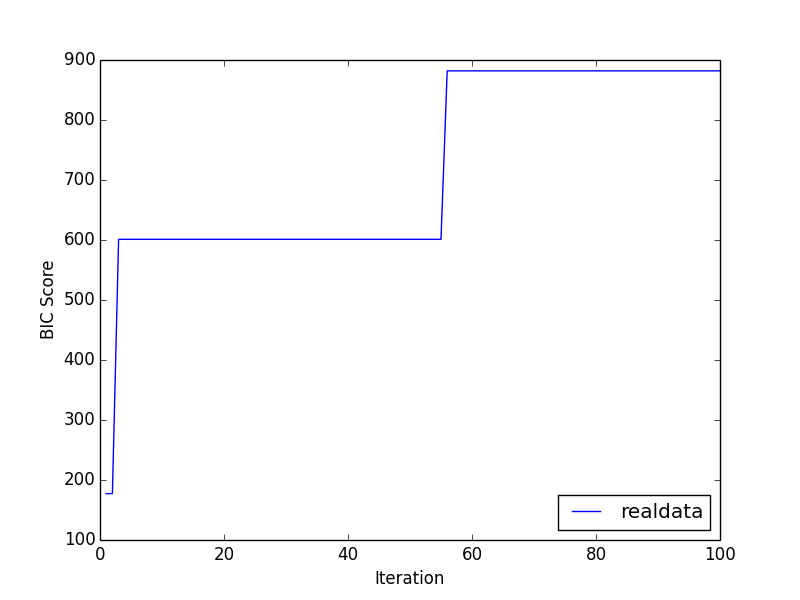
\includegraphics[height=8cm]{images/real_data}
		\caption{BIC Score (em milhares) para os dados reais}
		\label{fig:busca}
	\end{figure}
	Se são comparados os valores com os que tinha na subseção~\ref{subsec:exp1}, estos valores são muito maiores o que quer dizer que possivelmente tem uma maior quantidade de aristas no grafo. Ao final da execução do algoritmo, foi encontrada a rede mostrada na figura~\ref{fig:bestnet}.
	\begin{figure}[H]
		\centering
		\begin{tikzpicture}
	\tikzset{ vertex/.style = { shape = circle , draw , minimum size = 2.5em } }
	\tikzset{ edge/.style = { ->,> = latex' } }
	% vertices
	\node[ vertex ] (CG) at ( 4.5 , 0 ) { ${CG}$ } ;

	\node[ vertex ] (CL) at ( 0 , -2 ) { ${CL}$ } ;
	\node[ vertex ] (AI) at ( 3 , -2 ) { ${AI}$ } ;
	\node[ vertex ] (EN) at  ( 6 , -2 ) { ${EN}$ } ;
	\node[ vertex ] (W) at ( 9 , -2 ) { ${W}$ } ;
	
	\node[ vertex ] (S) at  ( 3 , -4 ) { ${S}$ } ;
	\node[ vertex ] (RA) at ( 6 , -4 ) { ${RA}$ } ;
	
	\node[ vertex ] (RE) at ( 0 , -6 ) { ${RE}$ } ;
	\node[ vertex ] (ED) at ( 3 , -6 ) { ${ED}$ } ;
	\node[ vertex ] (N) at  ( 6 , -6 ) { ${N}$ } ;
	\node[ vertex ] (H) at ( 9 , -6 ) { ${H}$ } ;
	
	\node[ vertex ] (M) at ( 6 , -8 ) { ${M}$ } ;
	\node[ vertex ] (AG) at  ( 9 , -8 ) { ${AG}$ } ;	
	\node[ vertex ] (O) at ( 3 , -8 ) { ${O}$ } ;
	
	%edges
	%age:
	%workclass:relationship, occupation
	\draw[ edge ] (W) to[out=-90,in=45] (RE) ;
	%\draw[ edge ] (W) to (O) ;
	%education:relationship, marital-status
	\draw[ edge ] (ED) to (RE) ;
	\draw[ edge ] (ED) to (M) ;
	%education-num:race, sex
	\draw[ edge ] (EN) to (RA) ;
	\draw[ edge ] (EN) to (S) ;
	%marital-status:occupation
	\draw[ edge ] (M) to (O) ;
	%occupation:
	%relationship:marital-status
	\draw[ edge ] (RE) to (M) ;
	%race:capital-loss, hours-per-week, sex, native-country, workclass
	%\draw[ edge ] (RA) to (CL) ;
	\draw[ edge ] (RA) to (H) ;
	\draw[ edge ] (RA) to (S) ;
	\draw[ edge ] (RA) to (N) ;
	\draw[ edge ] (RA) to (W) ;
	%sex:native-country
	\draw[ edge ] (S) to (N) ;
	%capital-gain:annual-income, education-num, race, capital-loss, hours-per-week, age, workclass
	\draw[ edge ] (CG) to (AI) ;
	\draw[ edge ] (CG) to (EN) ;
	%\draw[ edge ] (CG) to (RA) ;
	\draw[ edge ] (CG) to (CL) ;
	%\draw[ edge ] (CG) to (H) ;
	%\draw[ edge ] (CG) to (AG) ;
	\draw[ edge ] (CG) to (W) ;
	%capital-loss:hours-per-week, education, relationship
	%\draw[ edge ] (CL) to (H) ;
	\draw[ edge ] (CL) to (ED) ;
	\draw[ edge ] (CL) to (RE) ;
	%hours-per-week:native-country, age, education, marital-status
	\draw[ edge ] (H) to (N) ;
	\draw[ edge ] (H) to (AG) ;
	\draw[ edge ] (H) to[in=-30,out=-150] (ED) ;
	\draw[ edge ] (H) to (M) ;
	%native-country:age, workclass, education, occupation
	\draw[ edge ] (N) to (AG) ;
	%\draw[ edge ] (N) to (W) ;
	\draw[ edge ] (N) to (ED) ;
	\draw[ edge ] (N) to (O) ;
	%annual-income:education-num, race, capital-loss, sex
	%\draw[ edge ] (AI) to (EN) ;
	\draw[ edge ] (AI) to (RA) ;
	\draw[ edge ] (AI) to (CL) ;
	\draw[ edge ] (AI) to (S) ;
\end{tikzpicture}
		\caption{Melhor rede encontrada para o conjunto de dados}
		\label{fig:bestnet}
	\end{figure}
	O valor do parâmetro Data Log-Likelihood para esta rede é $DLL = -156842.48$ que é só um pouco maior à rede 1 feita manualmente.
\clearpage